\documentclass[11pt,xcolor=table]{beamer}

\usetheme[progressbar=frametitle]{metropolis}
\usepackage{appendixnumberbeamer}
\usepackage{pgfpages}
%\setbeameroption{show notes on second screen}
  \setbeamertemplate{enumerate items}[square]
\usepackage{multirow}

\usepackage{graphicx}

\usepackage{xcolor}

\newcommand{\link}[3][mLightBrown]{\href{#2}{\color{#1}{#3}}}%


\newcommand{\questionslide}[0]{
{\setbeamercolor{palette primary}{fg=black, bg=yellow}
\begin{frame}[standout]
    \raggedright
  Any questions? \\ \vspace{1cm}
  \raggedleft
  \dots{ } Remember -- Every question is useful!
\end{frame}
}}

\newcommand{\task}[1]{
   \begin{alertblock}
   {\centering \vspace{-1.5ex} \\ #1  \\ \vspace{-1.5ex} }
   \end{alertblock}
   }

\setbeamercolor{block title alerted}{%
    use={block title, alerted text},
    bg=yellow,
    fg=black
}

\definecolor{peppermint}{RGB}{75, 161, 115}
%\definecolor{peppermint}{RGB}{75, 161, 115}


\setbeamercolor{alerted text}{fg=peppermint , bg= black}

\usepackage{booktabs}
\usepackage[scale=2]{ccicons}

\usepackage{pgfplots}
\usepgfplotslibrary{dateplot}

\makeatletter 
\def\beamer@framenotesbegin{% at beginning of slide
    \usebeamercolor[fg]{normal text}
    \gdef\beamer@noteitems{}% 
    \gdef\beamer@notes{}% 
}
\makeatother


\usepackage{xspace}
\newcommand{\themename}{\textbf{\textsc{metropolis}}\xspace}

\title{From Diff in Diff to Panel Data
}
\subtitle{Econ 140, Section 11}
% \date{\today}
\date{}
\author{Jonathan Old}

% \titlegraphic{\hfill\includegraphics[height=1.5cm]{logo.pdf}}

\begin{document}

\maketitle

\begin{frame}{Roadmap}
  \setbeamertemplate{section in toc}[sections numbered]
  \tableofcontents%[hideallsubsections]
\end{frame}







\section{Recap: DiD}





\begin{frame}{How to get the causal effect of a treatment: DiD}


\begin{table}[]
\begin{tabular}{lcc}
\toprule
\textbf{}                        & \textbf{2020} & \textbf{2022} \\ \midrule
Free Mental Health: Treated      &    6       & 6          \\ \midrule
No Free Mental Health: Untreated &    4       & 5        \\ \bottomrule
\end{tabular}
\end{table}

We can do several comparisons:
\begin{itemize}[<+- | alert@+>]
\item Comparison 3: Compare treated to untreated group, before and after the intervention. \textbf{Differences in differences!}
\item Estimated treatment effect? $(6-6)-(5-4)=(6-5)-(6-4)=-1$
\item Identifying assumption: Parallel trends: Without the treatment, the average increase in the outcome of the treated would have been the same as the average increase in the outcome of the untreated.
\end{itemize} 
\end{frame}








\begin{frame}{Parallel trends assumption}

\begin{figure}
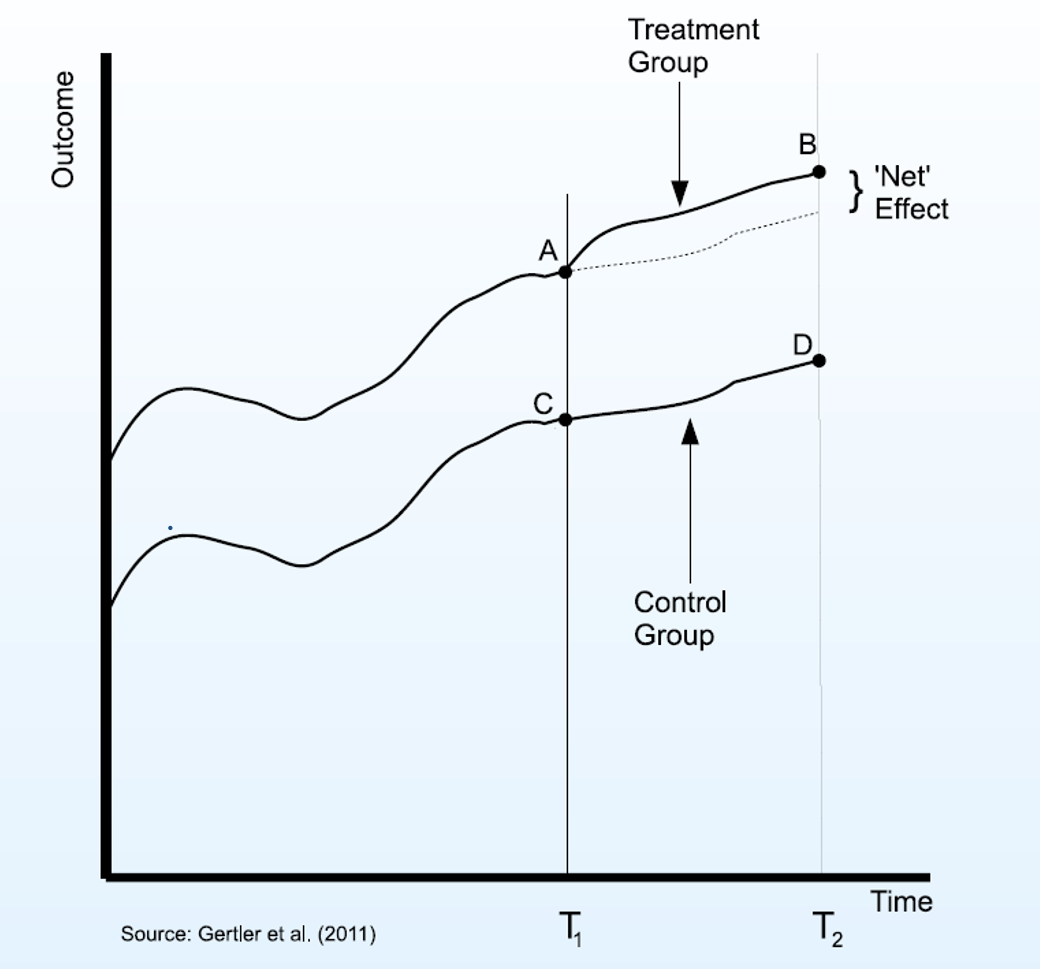
\includegraphics[width=0.8\textwidth]{figures/did1.png}
\end{figure}

\end{frame}




\begin{frame}{(Potential) violation of a parallel trends assumption}

\begin{figure}
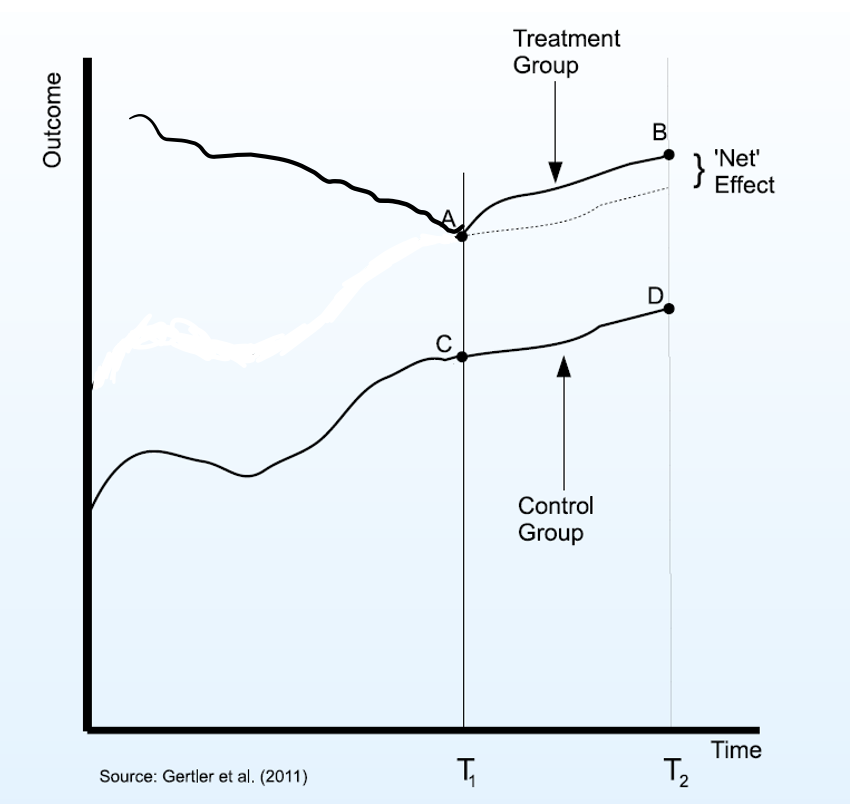
\includegraphics[width=0.8\textwidth]{figures/did2.png}
\end{figure}

\end{frame}






\begin{frame}{Estimating DiD with regressions}
We can set up a simple linear regression to estimate a  DiD model:
$$
Y_{i t}=\alpha+\beta \text { Treated }_i+\gamma \text { Post }_t+\delta \text { Treated }_i \cdot \text { Post }_t+u_{i t}
$$



\begin{table}[]
\begin{tabular}{lcc}
\toprule
\textbf{}                        & \textbf{2020} & \textbf{2022} \\ \midrule
Free Mental Health: Treated      &    $\alpha + \beta$       & $\alpha + \beta + \gamma + \delta$          \\ \midrule
No Free Mental Health: Untreated &    $\alpha$       & $\alpha + \gamma$        \\ \bottomrule
\end{tabular}
\end{table}


\end{frame}



\questionslide

\section{Making DiD more general: Panel Data estimation}




\begin{frame}{Limitations of the 2x2 DiD framework}
In the simple 2x2 framework, we estimated:
$$
Y_{i t}=\alpha+\beta \text { Treated }_i+\gamma \text { Post }_t+\delta \text { Treated }_i \cdot \text { Post }_t+u_{i t}
$$


How can we extend this framework?
% Only 2 groups, only two time periods, only discrete treatment, no controls

\end{frame}




\begin{frame}[allowframebreaks]{Intro to Panel Data}

A panel dataset may look like this:

\begin{figure}
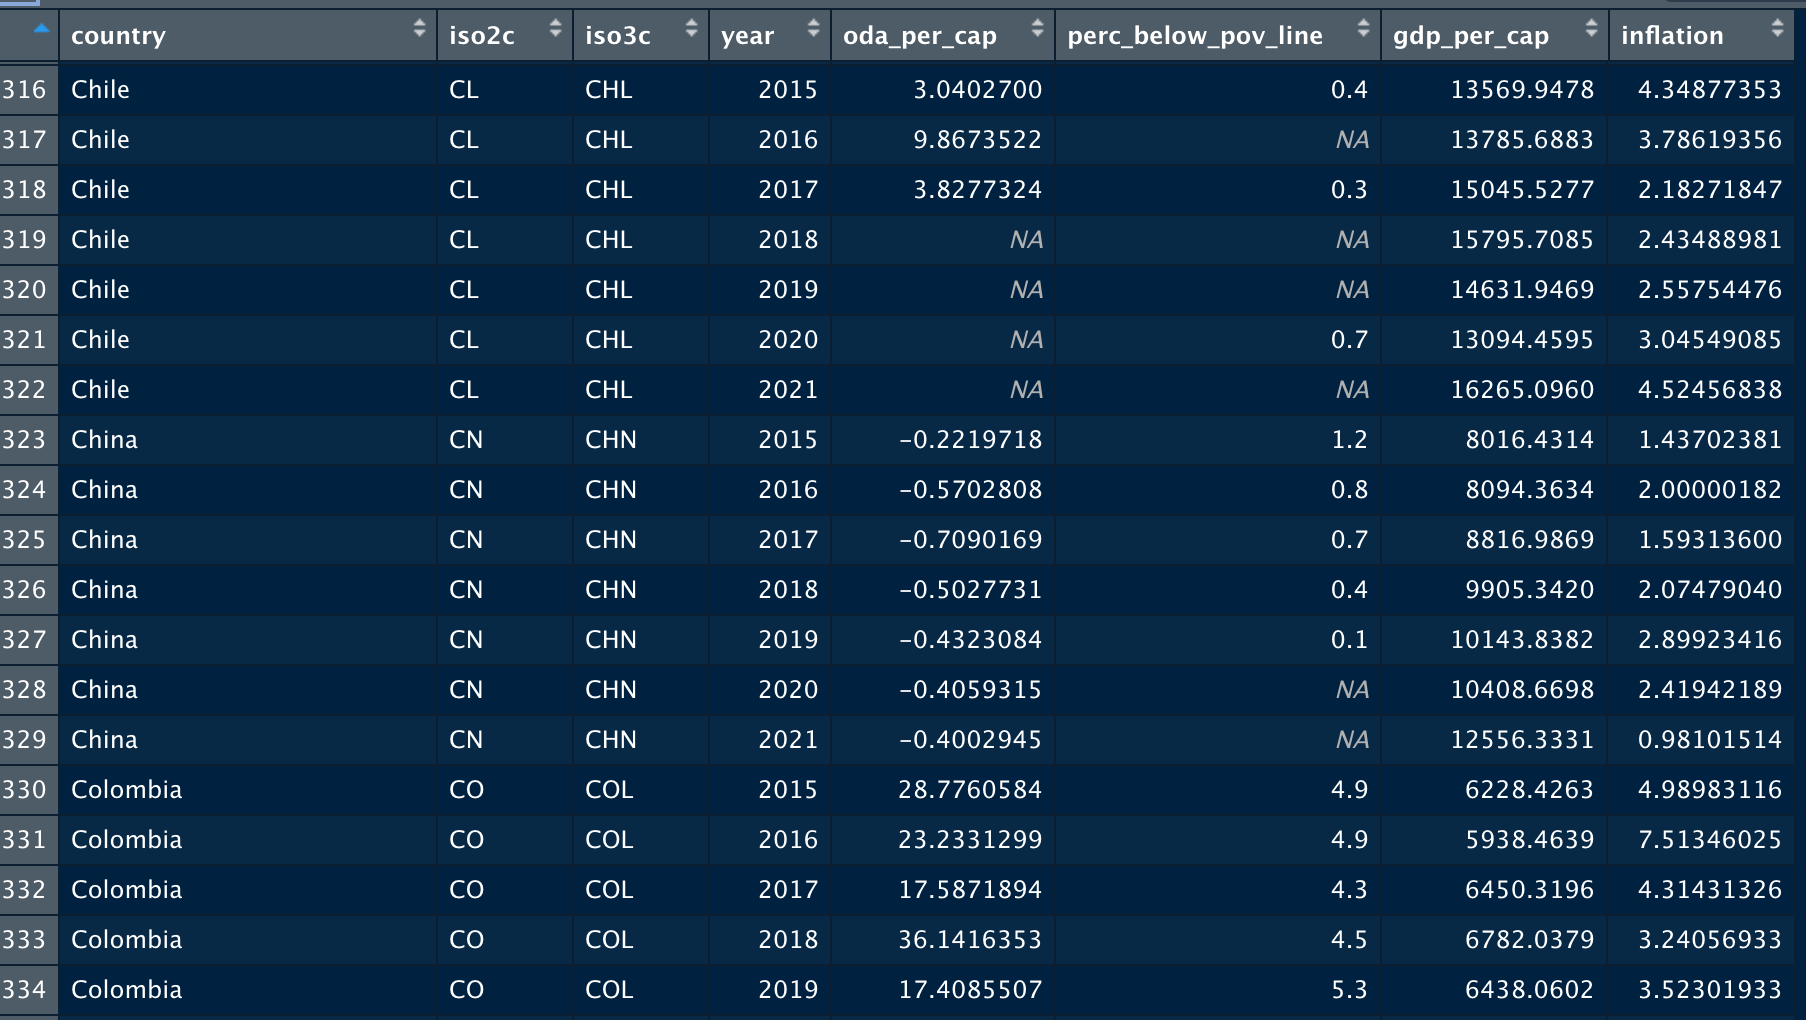
\includegraphics[width=0.9\textwidth]{figures/panel_long.png}
\end{figure}

\framebreak 

It may also look like this: 
\begin{figure}
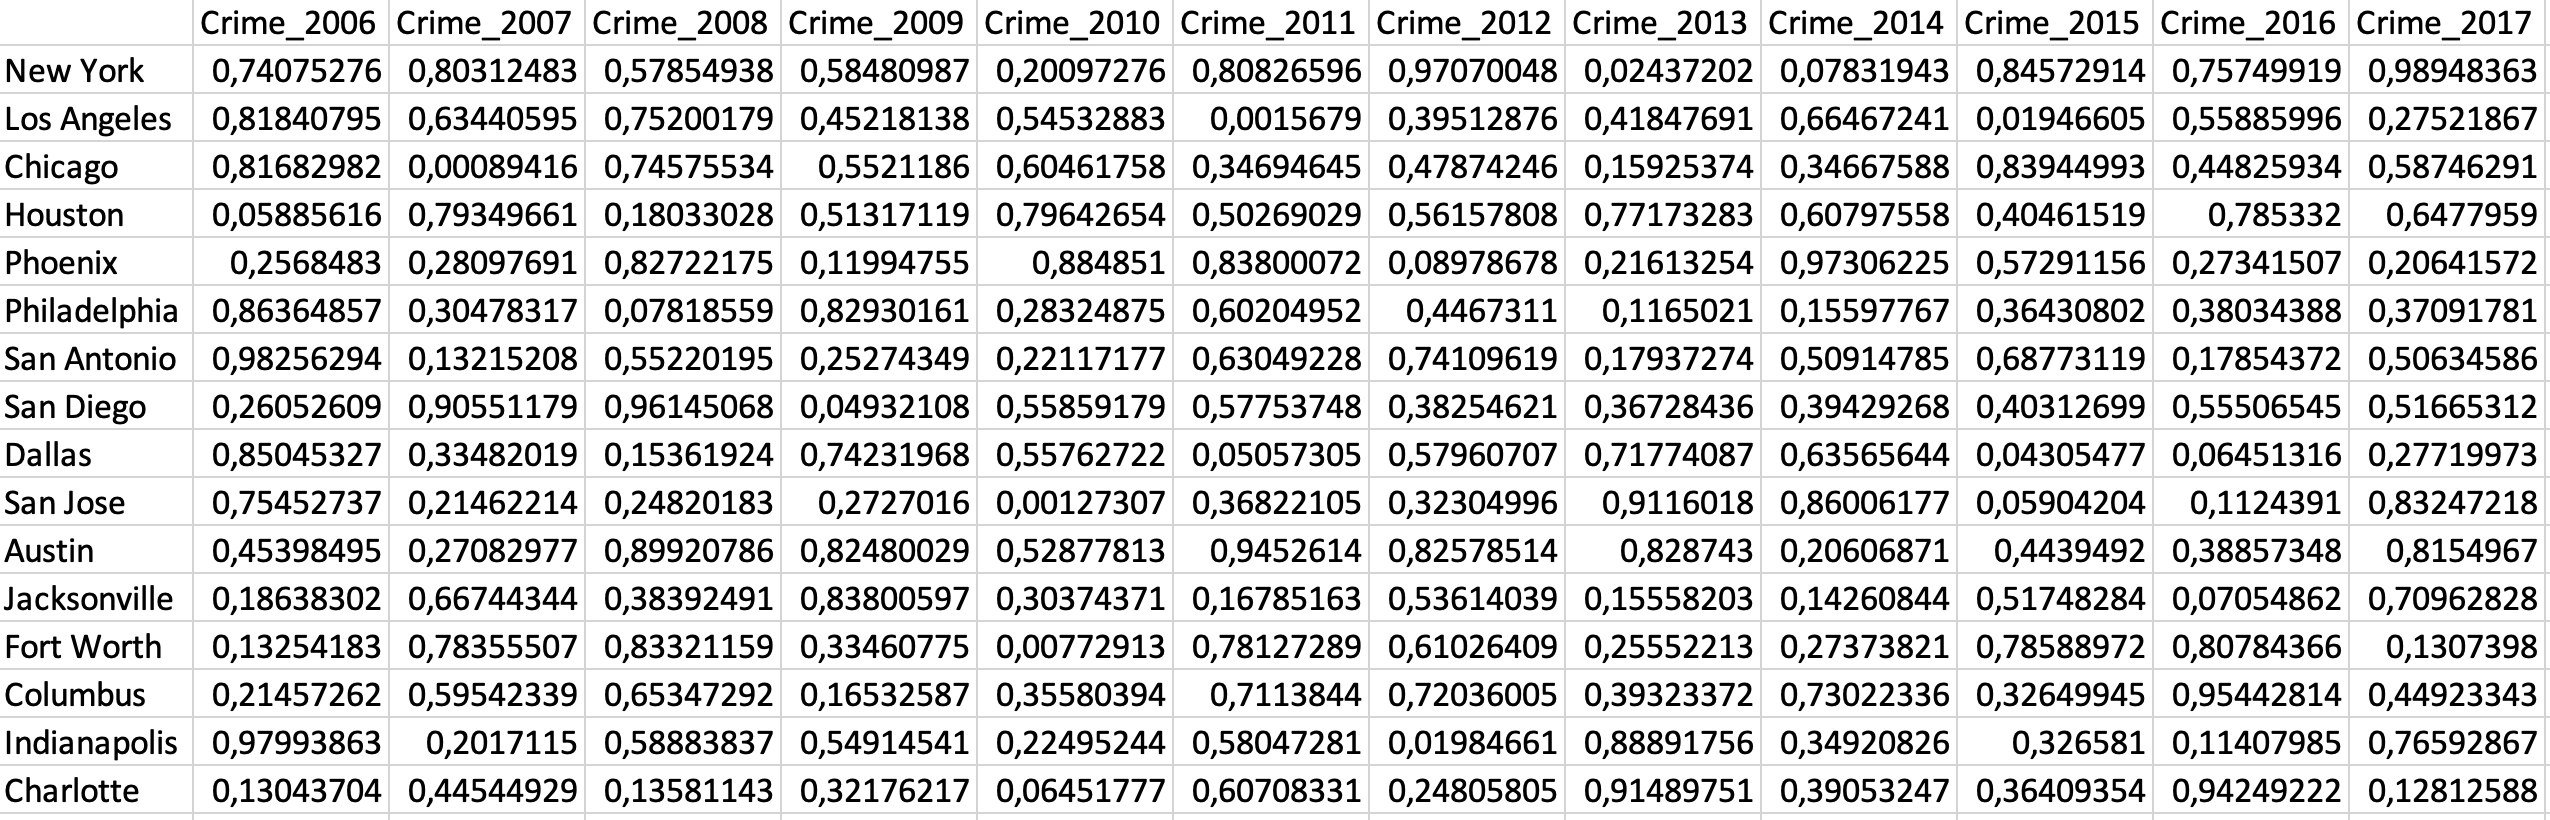
\includegraphics[width=1.0\textwidth]{figures/panel_wide.png}
\end{figure}
\end{frame}






\begin{frame}{Interpreting FE regressions}
Suppose we collect yearly data on firms' profits and the gender of the firms' CEO, for a sample of 1,000 firms over 20 years.

We can estimate this model with firm and year fixed effects:

$$ \text{Profits}_{i t}=\beta_0+\beta_1 \text{Female CEO}_{i t}+\alpha_i+\delta_t + \varepsilon_{i t} $$

How do we interpret $\beta_1$?

\pause 
The same way as in an OLS regression!

$\beta_1$ describes how having a female CEO is associated with profits, holding constant all firm-specific factors that do not change over time, and all time-specific factors that affect all firms equally.  $\beta_1$ is the effect within each firm (and year!), controlling for the firm-specific and year-specific fixed effects.


\end{frame}




\begin{frame}{Visualization}

See separate \alert{\textbf{\href{https://jonathanold.github.io/images/fe.gif}{gif}}}!

\end{frame}





\begin{frame}{Limitations of fixed effects}


\begin{itemize}
\item Imagine we want to estimate the effect of annual income on happiness and we have a panel following 1,000 individuals over 10 years. You think there are many omitted variables and include individual-level fixed effects. You are \textbf{also} interested in the effect of parental income on happiness. What's the problem?
\pause 
\item We want to estimate the effect of democracy on economic growth in a panel of 180 countries over 60 years. We can include country-fixed effects to account for any effect coming from different countries having a different climate, terrain, access to the sea, culture, etc. Are you satisfied with this approach?
\pause 
\item We want to estimate the effect of education on wages and think of using individual-level fixed effects. What can go wrong?


\end{itemize}


\end{frame}


\questionslide




\section{Practice question}


\begin{frame}

\small
Did Welfare Reform Increase Employment?
In the 1990s, in an effort known as 'Welfare Reform' the United States implemented a series of policies that aimed to reduce welfare dependency by incentivizing work and raising the hassle of being on welfare. These reforms were implemented at the state level between 1993 and 1997. In this exercise, you will investigate whether welfare reform successfully raised employment rates.

The file welfare.csv contains information on individuals in the U.S. between 1990 and 2005. The key variables are

\begin{itemize}
\item employed: dummy equal to one if individual is employed
\item reform: dummy equal to one if the individual is living in a state that has welfare reform in place in that year
\item hsgrad: dummy equal to one if individual has a HS degree
\item white: dummy equal to one if individual is white
\item woman: dummy equal to one if individual identifies as a woman
\item avg\_benefit: the average welfare benefit (between 1990 and 2005) for a family of three in that individual's state
\end{itemize}


\end{frame}


\begin{frame}
Estimate a regression of
(1) employed against reform
(2) employed against reform, hsgrad, white, and woman and interpret the coefficient on reform in both regressions.
\end{frame}


\begin{frame}
Suggest a variable that varies across states but plausibly varies little-or not at all-over time and that could cause omitted variable bias in regression (2).

Estimate regression (2) using state fixed effects. How does the coefficient change? What does this suggest about the ommitted variable bias in part (b)? Which omitted variables do we account for with state FE?

Estimate regression (2) using time fixed effects. Interpret the interpret the coefficient on reform. How does the coefficient change? What does this suggest about the ommitted variable bias in part (b)? Which omitted variables do we account for with time FE?

\end{frame}



\begin{frame}

Estimate regression (2) using time AND state fixed effects. Interpret the interpret the coefficient on reform. How does the coefficient change? What does this suggest about the ommitted variable bias in part (b)? Which omitted variables do we account for with state and time FE?

Which specification (no FE, state FE, time FE, or state + time FE) is most credible and why?
\end{frame}

\begin{frame}{See you on R!}

\end{frame}












 









\end{document}
